% Options for packages loaded elsewhere
\PassOptionsToPackage{unicode}{hyperref}
\PassOptionsToPackage{hyphens}{url}
\PassOptionsToPackage{dvipsnames,svgnames,x11names}{xcolor}
%
\documentclass[
]{article}

\usepackage{amsmath,amssymb}
\usepackage{iftex}
\ifPDFTeX
  \usepackage[T1]{fontenc}
  \usepackage[utf8]{inputenc}
  \usepackage{textcomp} % provide euro and other symbols
\else % if luatex or xetex
  \usepackage{unicode-math}
  \defaultfontfeatures{Scale=MatchLowercase}
  \defaultfontfeatures[\rmfamily]{Ligatures=TeX,Scale=1}
\fi
\usepackage{lmodern}
\ifPDFTeX\else  
    % xetex/luatex font selection
\fi
% Use upquote if available, for straight quotes in verbatim environments
\IfFileExists{upquote.sty}{\usepackage{upquote}}{}
\IfFileExists{microtype.sty}{% use microtype if available
  \usepackage[]{microtype}
  \UseMicrotypeSet[protrusion]{basicmath} % disable protrusion for tt fonts
}{}
\makeatletter
\@ifundefined{KOMAClassName}{% if non-KOMA class
  \IfFileExists{parskip.sty}{%
    \usepackage{parskip}
  }{% else
    \setlength{\parindent}{0pt}
    \setlength{\parskip}{6pt plus 2pt minus 1pt}}
}{% if KOMA class
  \KOMAoptions{parskip=half}}
\makeatother
\usepackage{xcolor}
\usepackage[left=1in,right=1in]{geometry}
\setlength{\emergencystretch}{3em} % prevent overfull lines
\setcounter{secnumdepth}{-\maxdimen} % remove section numbering
% Make \paragraph and \subparagraph free-standing
\makeatletter
\ifx\paragraph\undefined\else
  \let\oldparagraph\paragraph
  \renewcommand{\paragraph}{
    \@ifstar
      \xxxParagraphStar
      \xxxParagraphNoStar
  }
  \newcommand{\xxxParagraphStar}[1]{\oldparagraph*{#1}\mbox{}}
  \newcommand{\xxxParagraphNoStar}[1]{\oldparagraph{#1}\mbox{}}
\fi
\ifx\subparagraph\undefined\else
  \let\oldsubparagraph\subparagraph
  \renewcommand{\subparagraph}{
    \@ifstar
      \xxxSubParagraphStar
      \xxxSubParagraphNoStar
  }
  \newcommand{\xxxSubParagraphStar}[1]{\oldsubparagraph*{#1}\mbox{}}
  \newcommand{\xxxSubParagraphNoStar}[1]{\oldsubparagraph{#1}\mbox{}}
\fi
\makeatother


\providecommand{\tightlist}{%
  \setlength{\itemsep}{0pt}\setlength{\parskip}{0pt}}\usepackage{longtable,booktabs,array}
\usepackage{calc} % for calculating minipage widths
% Correct order of tables after \paragraph or \subparagraph
\usepackage{etoolbox}
\makeatletter
\patchcmd\longtable{\par}{\if@noskipsec\mbox{}\fi\par}{}{}
\makeatother
% Allow footnotes in longtable head/foot
\IfFileExists{footnotehyper.sty}{\usepackage{footnotehyper}}{\usepackage{footnote}}
\makesavenoteenv{longtable}
\usepackage{graphicx}
\makeatletter
\def\maxwidth{\ifdim\Gin@nat@width>\linewidth\linewidth\else\Gin@nat@width\fi}
\def\maxheight{\ifdim\Gin@nat@height>\textheight\textheight\else\Gin@nat@height\fi}
\makeatother
% Scale images if necessary, so that they will not overflow the page
% margins by default, and it is still possible to overwrite the defaults
% using explicit options in \includegraphics[width, height, ...]{}
\setkeys{Gin}{width=\maxwidth,height=\maxheight,keepaspectratio}
% Set default figure placement to htbp
\makeatletter
\def\fps@figure{htbp}
\makeatother

\makeatletter
\@ifpackageloaded{caption}{}{\usepackage{caption}}
\AtBeginDocument{%
\ifdefined\contentsname
  \renewcommand*\contentsname{Table of contents}
\else
  \newcommand\contentsname{Table of contents}
\fi
\ifdefined\listfigurename
  \renewcommand*\listfigurename{List of Figures}
\else
  \newcommand\listfigurename{List of Figures}
\fi
\ifdefined\listtablename
  \renewcommand*\listtablename{List of Tables}
\else
  \newcommand\listtablename{List of Tables}
\fi
\ifdefined\figurename
  \renewcommand*\figurename{Figure}
\else
  \newcommand\figurename{Figure}
\fi
\ifdefined\tablename
  \renewcommand*\tablename{Table}
\else
  \newcommand\tablename{Table}
\fi
}
\@ifpackageloaded{float}{}{\usepackage{float}}
\floatstyle{ruled}
\@ifundefined{c@chapter}{\newfloat{codelisting}{h}{lop}}{\newfloat{codelisting}{h}{lop}[chapter]}
\floatname{codelisting}{Listing}
\newcommand*\listoflistings{\listof{codelisting}{List of Listings}}
\makeatother
\makeatletter
\makeatother
\makeatletter
\@ifpackageloaded{caption}{}{\usepackage{caption}}
\@ifpackageloaded{subcaption}{}{\usepackage{subcaption}}
\makeatother

\ifLuaTeX
  \usepackage{selnolig}  % disable illegal ligatures
\fi
\usepackage{bookmark}

\IfFileExists{xurl.sty}{\usepackage{xurl}}{} % add URL line breaks if available
\urlstyle{same} % disable monospaced font for URLs
\hypersetup{
  pdftitle={Ethnic Enclaves and the Legacy of Internment},
  colorlinks=true,
  linkcolor={blue},
  filecolor={Maroon},
  citecolor={Blue},
  urlcolor={Blue},
  pdfcreator={LaTeX via pandoc}}


\title{Ethnic Enclaves and the Legacy of Internment}
\author{Dante Yasui}
\date{}

\begin{document}
\maketitle


\section{Intro}\label{intro}

\begin{center}
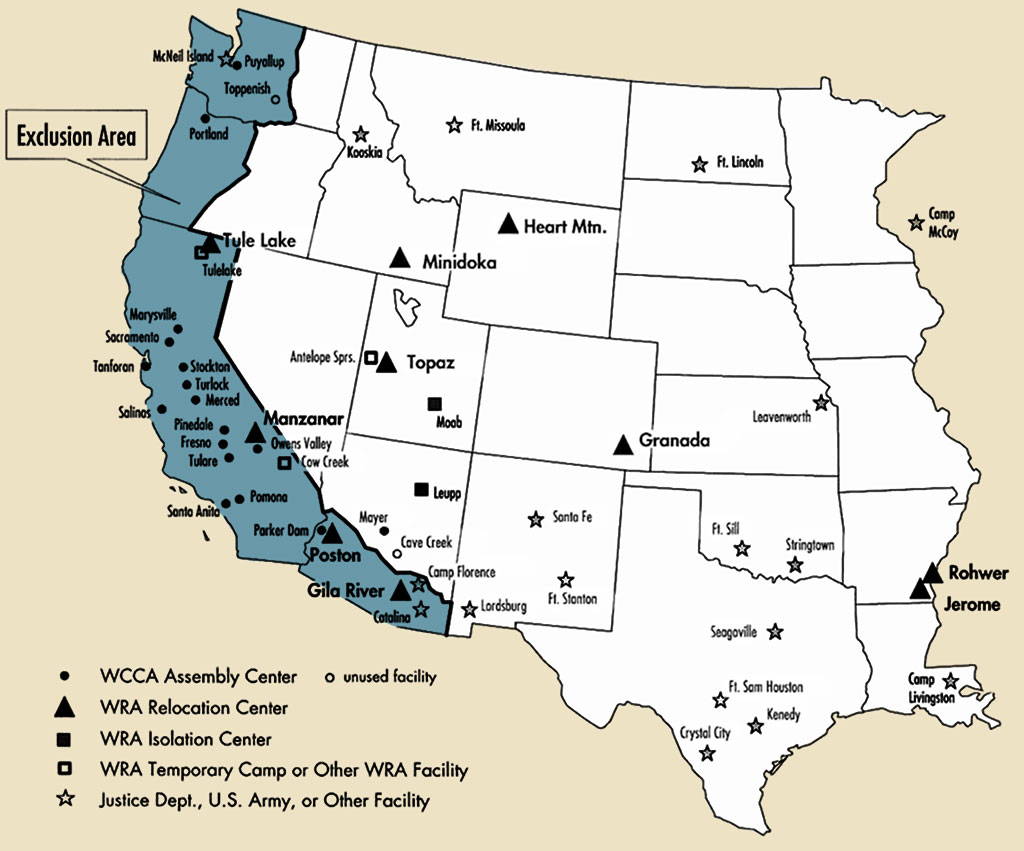
\includegraphics{figures/PioCrtInternmentMap.jpg}
\end{center}

\subsection{Research Question}\label{research-question}

\begin{itemize}
\tightlist
\item
  Did post-war relocation cause a permanent shift in the migration
  choices of Japanese Americans?
\end{itemize}

\begin{center}\rule{0.5\linewidth}{0.5pt}\end{center}

\subsection{Motivation}\label{motivation}

\begin{itemize}
\item
  Immigrant populations tend to concentrate near places of initial
  settlement
\item
  Integration/assimilation could be important for immigrant labor market
  outcomes

  \begin{itemize}
  \tightlist
  \item
    (\textbf{damm\_ethnic\_2009?})
  \end{itemize}
\item
  Evidence for Canadian Japanese internment having persistant effect on
  spatial Japanese distribution
\item
  (\textbf{chan\_forced\_2022?})
\end{itemize}

\subsection{Initial Distribution of pre-war Japanese
Population}\label{initial-distribution-of-pre-war-japanese-population}

\begin{center}
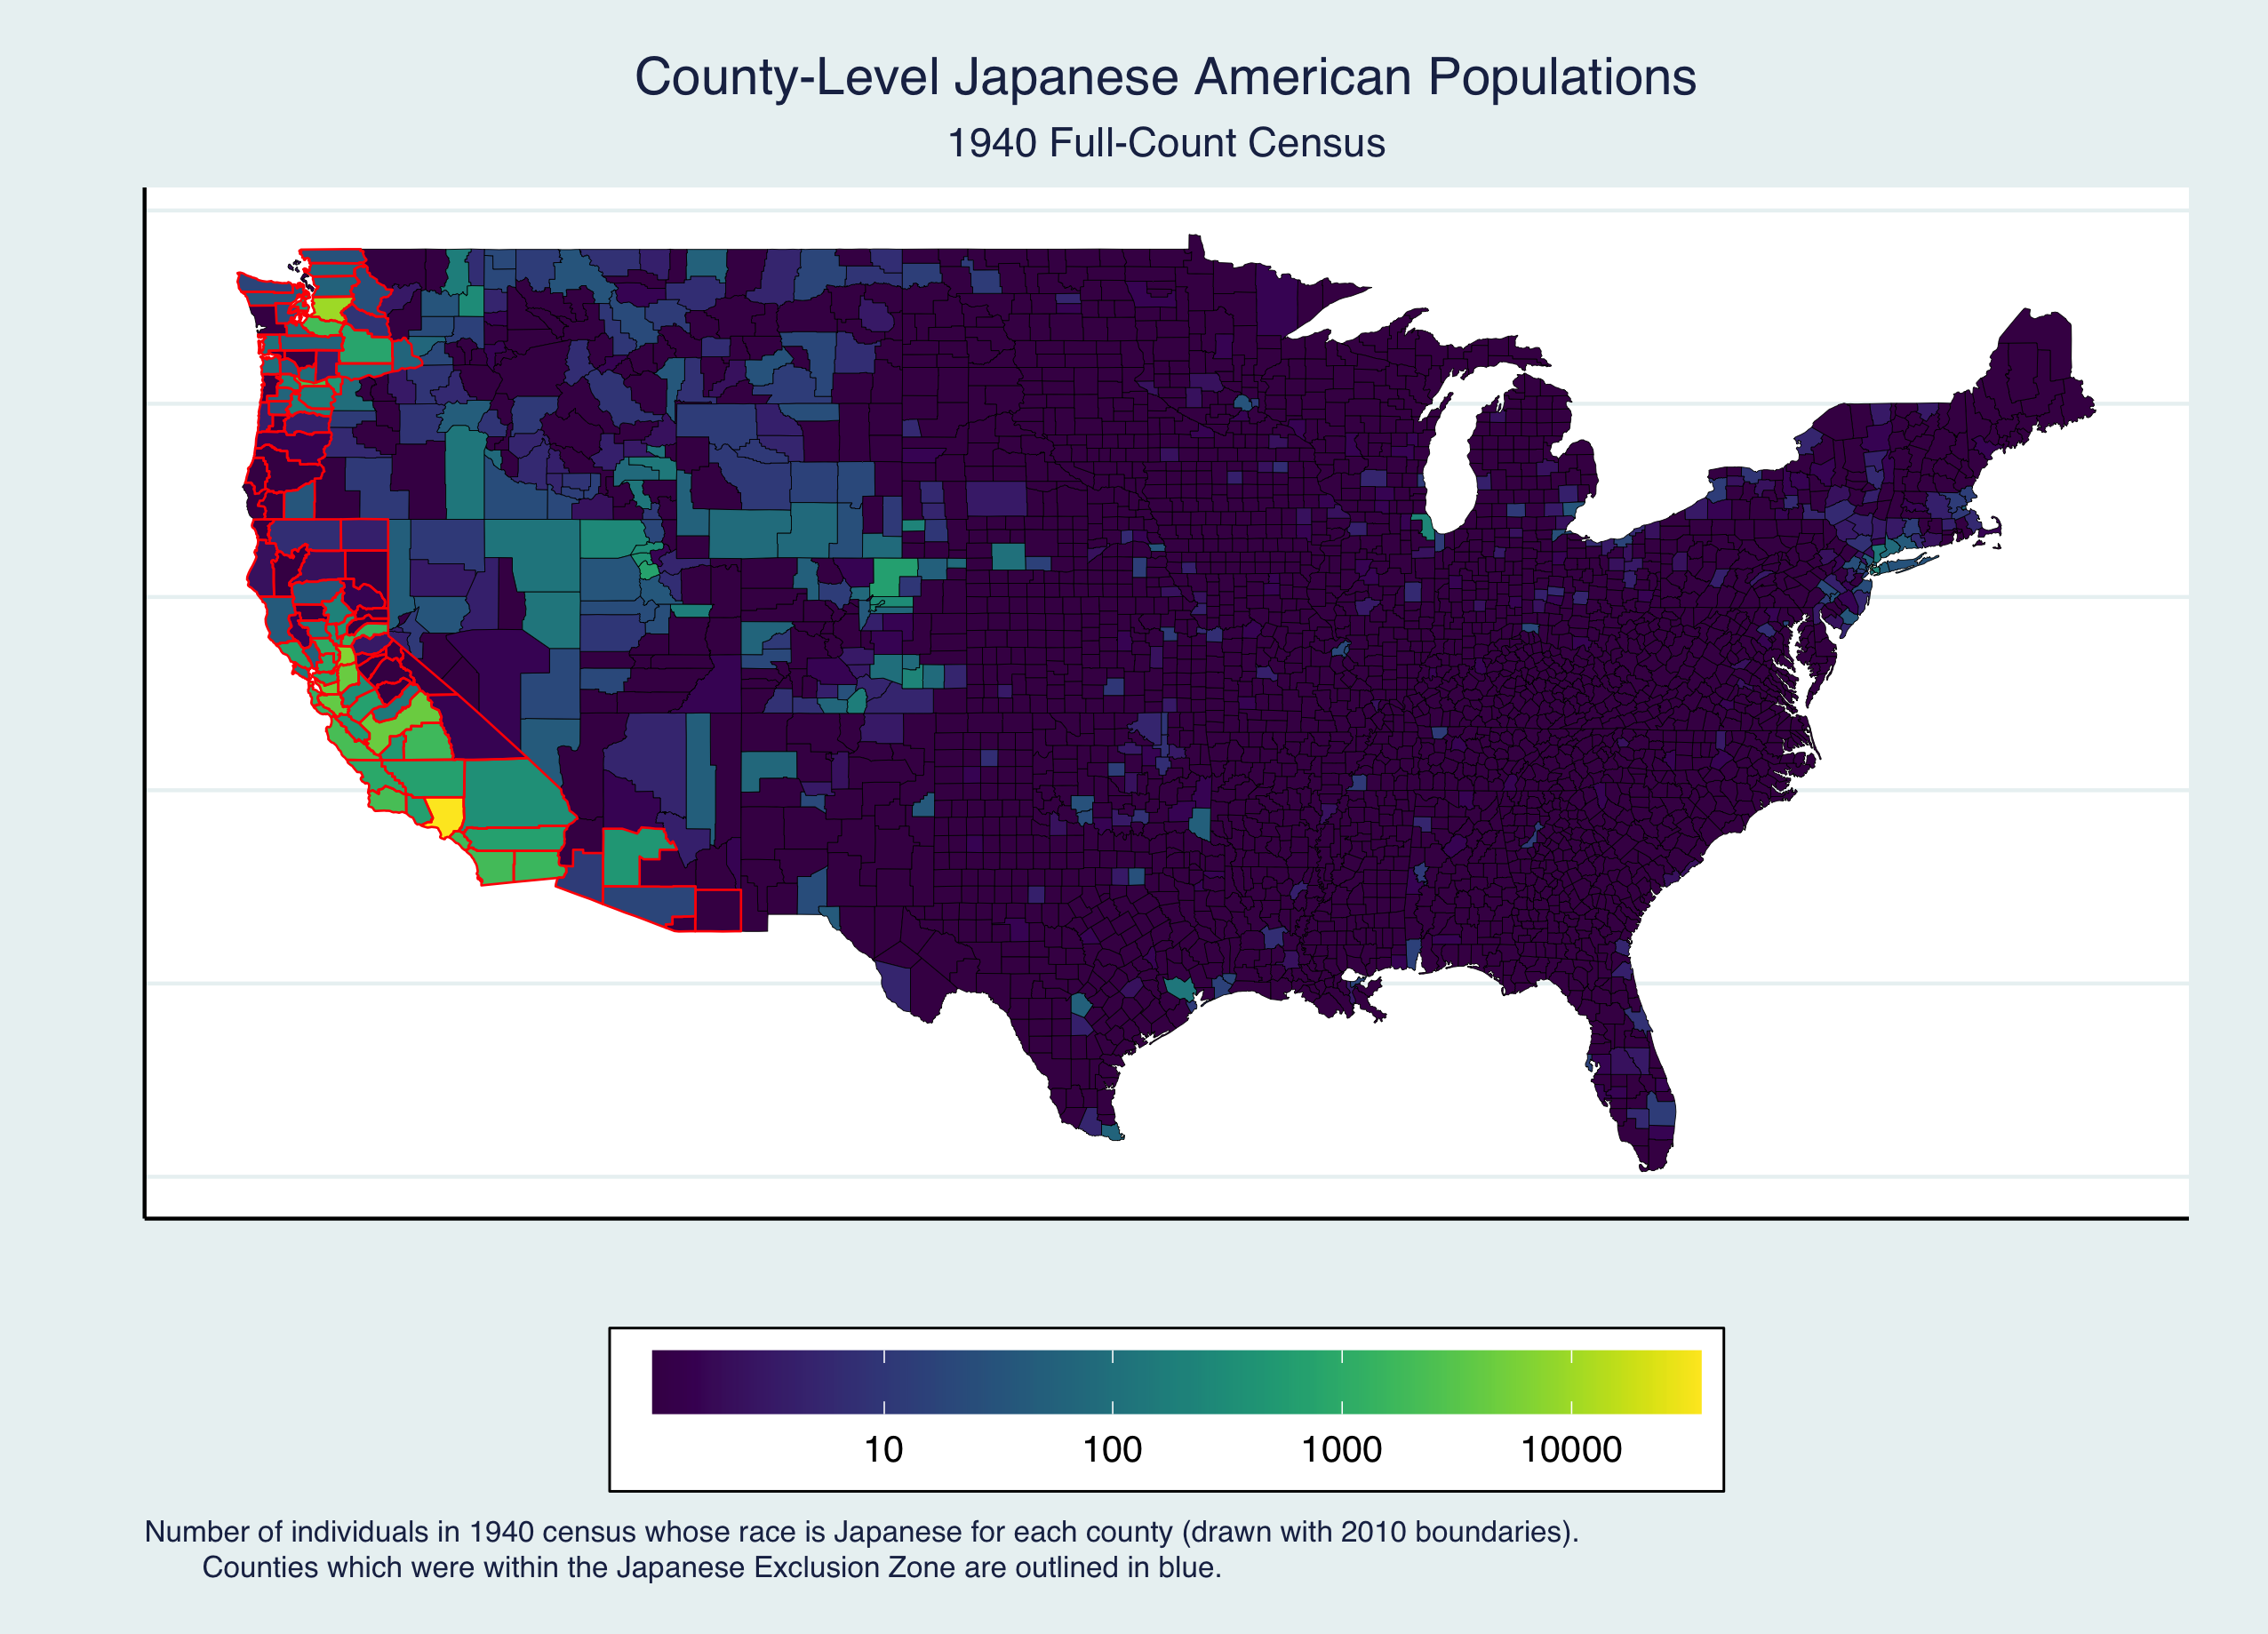
\includegraphics{figures/county_JAmap.png}
\end{center}

\subsection{Assignment of Internees to
Camps}\label{assignment-of-internees-to-camps}

\begin{center}
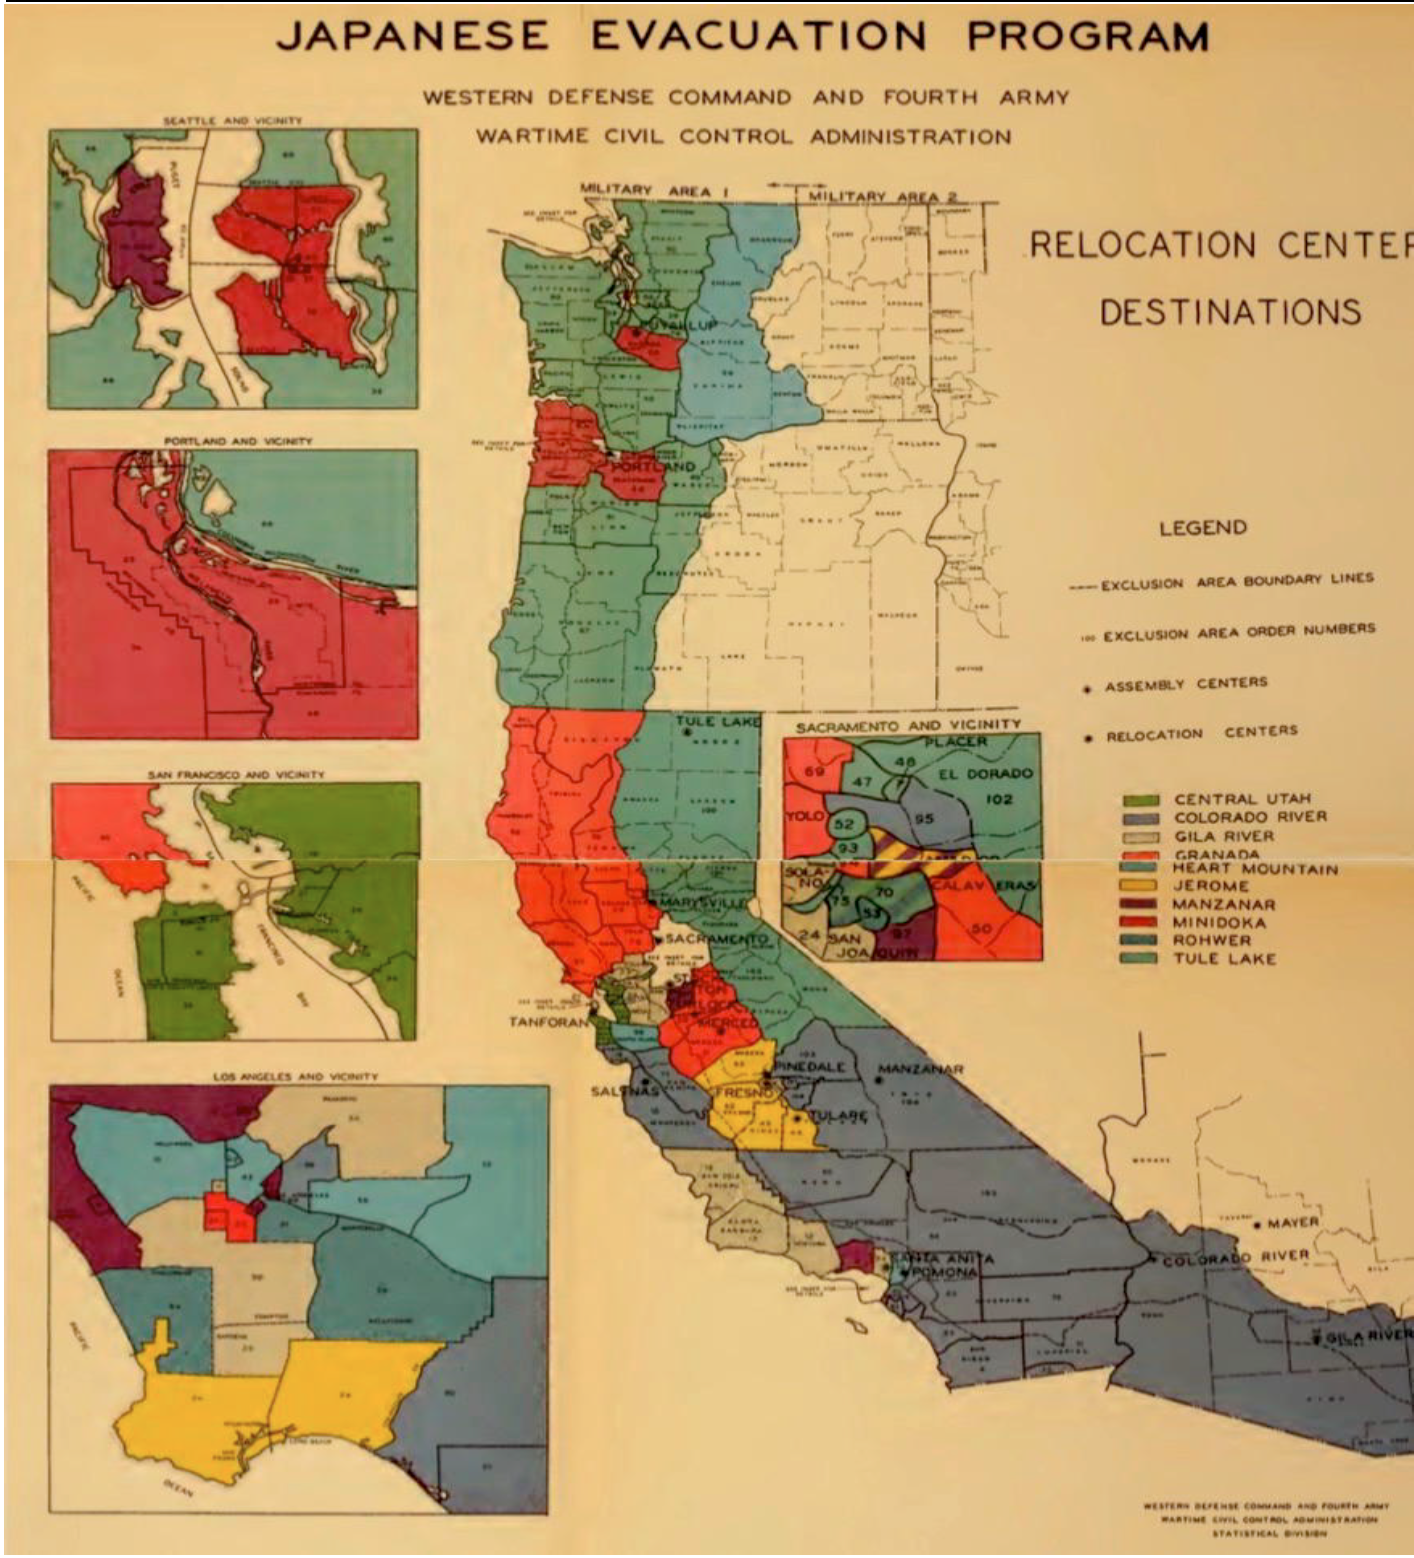
\includegraphics{figures/WRAzonesmap.png}
\end{center}

\begin{center}\rule{0.5\linewidth}{0.5pt}\end{center}

\section{Data}\label{data}

\textsubscript{Source:
\href{https://dyasui.github.io/FieldPaper_new/main.qmd.html}{Article
Notebook}}

\subsection{Population and Migration}\label{population-and-migration}

\textsubscript{Source:
\href{https://dyasui.github.io/FieldPaper_new/main.qmd.html}{Article
Notebook}}

For long-run migration data, I use the Decennial Census data provided by
the US Census Bureau via the
\href{https://usa.ipums.org/usa/index.shtml}{Integrated Public Use
Microdata Series} (\textbf{ruggles\_steven\_ipums\_2024?}). The census
samples for which county locations are available include the 1940, 1950,
1980, and 1990 1\% samples, the 1960 5\% sample, and the 1970 Form 2
Metro 1\% sample.

For the calculation of migration rates between counties, I define a
migrant as someone who reports that they either moved within the state,
between states, or that they were abroad five years ago (or in the past
1 year for 1960 respondants). This excludes people who report moving
within the same house, didn't report their previous location, or the
location is unknown.

\subsection{Geography}\label{geography}

\subsubsection{Historical County
Borders}\label{historical-county-borders}

\textsubscript{Source:
\href{https://dyasui.github.io/FieldPaper_new/main.qmd.html}{Article
Notebook}}

\textsubscript{Source:
\href{https://dyasui.github.io/FieldPaper_new/main.qmd.html}{Article
Notebook}}

\textsubscript{Source:
\href{https://dyasui.github.io/FieldPaper_new/main.qmd.html}{Article
Notebook}}

Although most county borders did not change much in the second half of
the 20th Century, there were counties which split, merged, or had name
changes which can make cross-decade comparisons difficult. For these
reasons, I choose to standardize the set of counties in my analysis to
the set of counties as they appear in the year 1990. To map historical
county-level data to 1990 county definitions, I implement the crosswalk
method by (\textbf{eckert\_method\_2020?}). They overlay historical
county boundary shapefiles from \href{NHGIS}{https://www.nhgis.org/}
onto county boundaries for a specific target year (in this case 1990).
The sub-areas created by these overlays are used to calculate a set of
geographic weights which represent the fractions of a 1990 county's area
which were within the geographic areas of counties as they appear in
different decades (specifically the decades between and including 1940
to 1980). For my analysis, I take the crosswalk weights from the example
csv file for the end year 1990 which is published on the authors'
\href{https://github.com/liang-jack-a/EGLP_Crosswalk/tree/master}{github
repository}.

\textsubscript{Source:
\href{https://dyasui.github.io/FieldPaper_new/main.qmd.html}{Article
Notebook}}

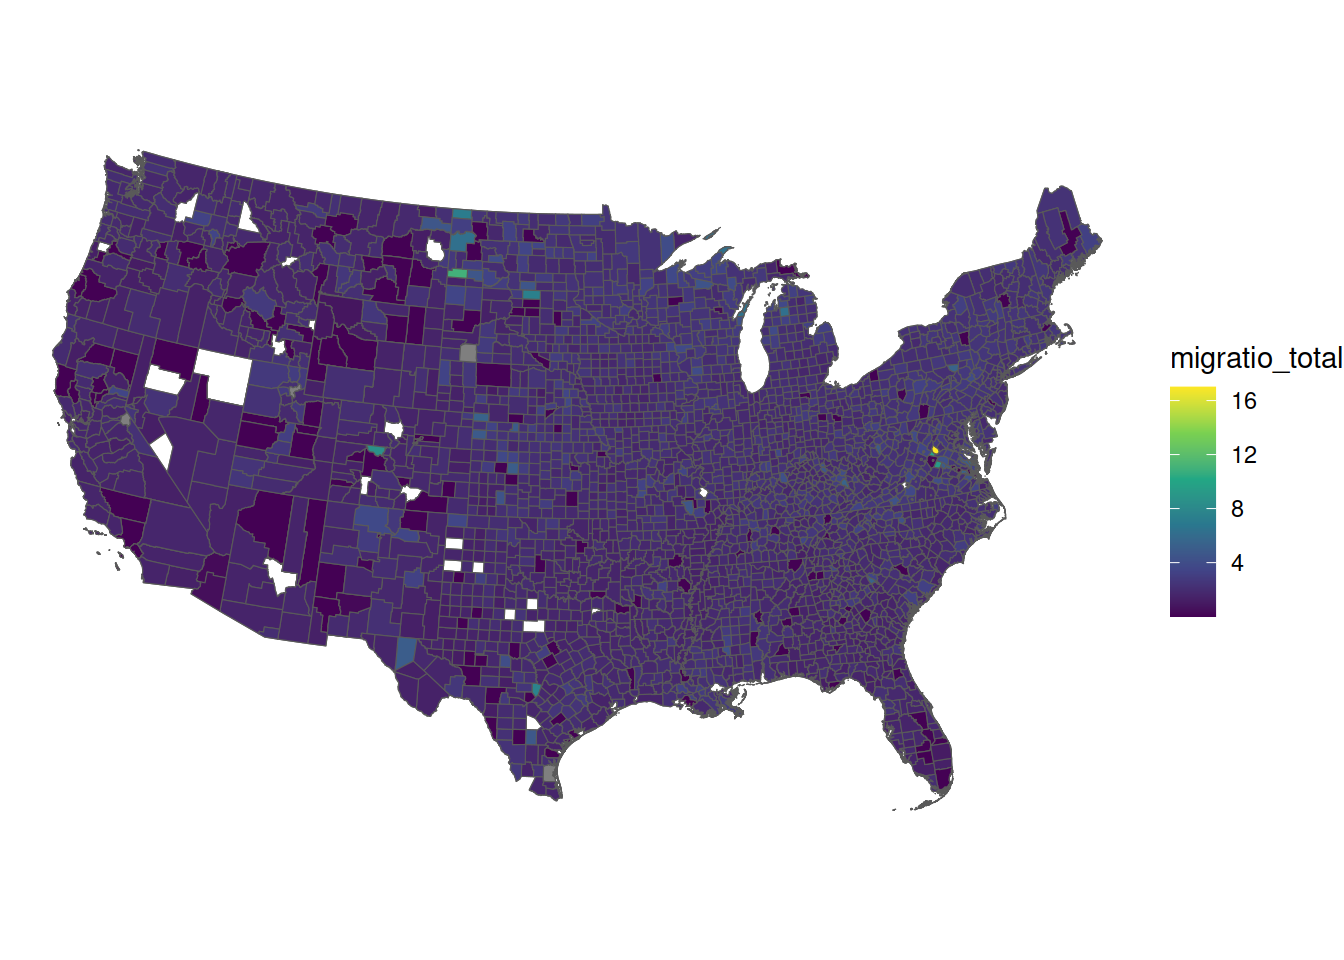
\includegraphics{main_files/figure-pdf/unnamed-chunk-1-1.pdf}

\textsubscript{Source:
\href{https://dyasui.github.io/FieldPaper_new/main.qmd.html}{Article
Notebook}}

\subsubsection{Camp Locations}\label{camp-locations}

Locations for historical interment camp locations were archived by
\href{http://encyclopedia.densho.org/War_Relocation_Authority/\#Planning_the_Camps}{Densho
Encyclopedia} and downloaded in csv form via the
\href{https://www.arcgis.com/home/item.html?id=69183af8d45d4f46a9dc4eba99440891}{Behind
Barbed Wires story project}.

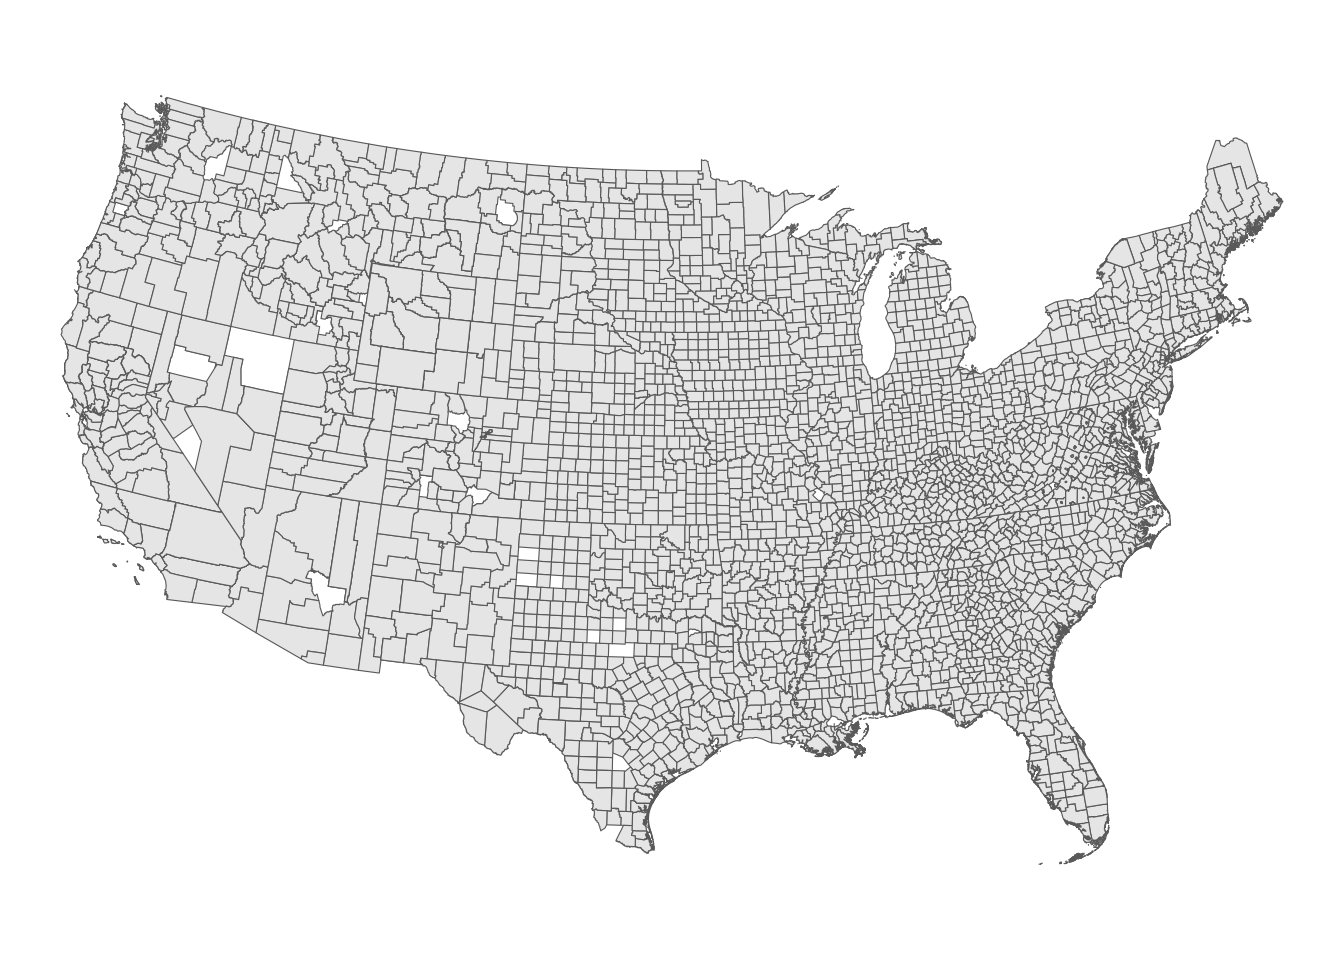
\includegraphics{main_files/figure-pdf/read-camplocations-1.pdf}

\textsubscript{Source:
\href{https://dyasui.github.io/FieldPaper_new/main.qmd.html}{Article
Notebook}}

I calculate the straight line distances in meters between each 1950
county centroid to each camp location in QGIS with the
\texttt{Distance\ Matrix} tool using the Standard (N x T) distance
matrix setting.

\textsubscript{Source:
\href{https://dyasui.github.io/FieldPaper_new/main.qmd.html}{Article
Notebook}}

\subsection{Historical counties
dataset}\label{historical-counties-dataset}

After narrowing down to counties which can be observed in each census
year and then translating the historical counties to 1990 county
boundaries, I am left with 3082 counties with observable migration rates
in 1940, 108 in 1950, 410 in 1960, 115 in 1970, 254 in 1980, and 290 in
1990.

My primary dataset is therefore a pooled-crossection with a total number
of 28 county-year level observations. Each observation represents an
individual county at a given year in time if it had the same borders as
it had in 1990.

The Census Bureau confidentiality standards state that public-use
microdata will cannot show report locations with populations of less
than 100,000 people. For this reason, many sparsely-populated counties
will be omitted from my sample because there are not enough observations
for the Census to report locations of individuals living there.

\textsubscript{Source:
\href{https://dyasui.github.io/FieldPaper_new/main.qmd.html}{Article
Notebook}}

\phantomsection\label{cell-fig-comparesamplepops}
\begin{figure}[H]

\centering{

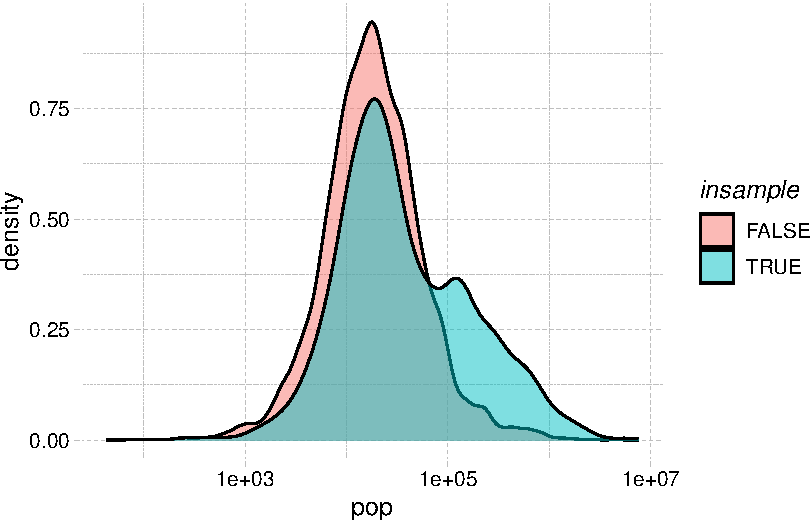
\includegraphics{main_files/figure-pdf/fig-comparesamplepops-1.pdf}

}

\caption{\label{fig-comparesamplepops}County-year level population
distributions}

\end{figure}%

\textsubscript{Source:
\href{https://dyasui.github.io/FieldPaper_new/main.qmd.html}{Article
Notebook}}

The average population of the census-year observations in my sample is
\ensuremath{1.3326856\times 10^{5}} while the average population for
crosswalked census-year observations outside my sample is
\ensuremath{3.9299349\times 10^{4}}. The fact that my sample is not
fully representative of all county sizes will be a challenge for the
external validity of my findings to extrapolate my results to smaller
counties for which I have less information on. However,
Figure~\ref{fig-comparesamplepops} shows that two different densities of
county-year populations observed in and out of the main sample have
similar shapes with the exception of a larger right-tail in the
in-sample density plot. This reflects the fact that counties with
populations of greater than 100,000 meet the Census Bureau's
confidentiality criteria, while data from smaller counties are subject
to stricter confidentiality measures.

\subsection{WRA first addresses}\label{wra-first-addresses}

\begin{itemize}
\tightlist
\item
  {\emph{The Evacuated People: A Quantitative Descripton}}
  (\textbf{krug\_evacuated\_1946?})

  \begin{itemize}
  \tightlist
  \item
    Final WRA report on ``State and Post Office Address of First
    Destination by Nativity, Prior January 1, 1945 and January 1, 1945
    and Later''
  \item
    Digitized and uploaded by Cooper Thomas via
    \href{https://data.world/infinitecoop/japanese-internment-camps}{data.world}
  \end{itemize}
\end{itemize}

\subsubsection{Map of Relocated Internees by
City}\label{map-of-relocated-internees-by-city}

\subsection{WRA internees}\label{wra-internees}

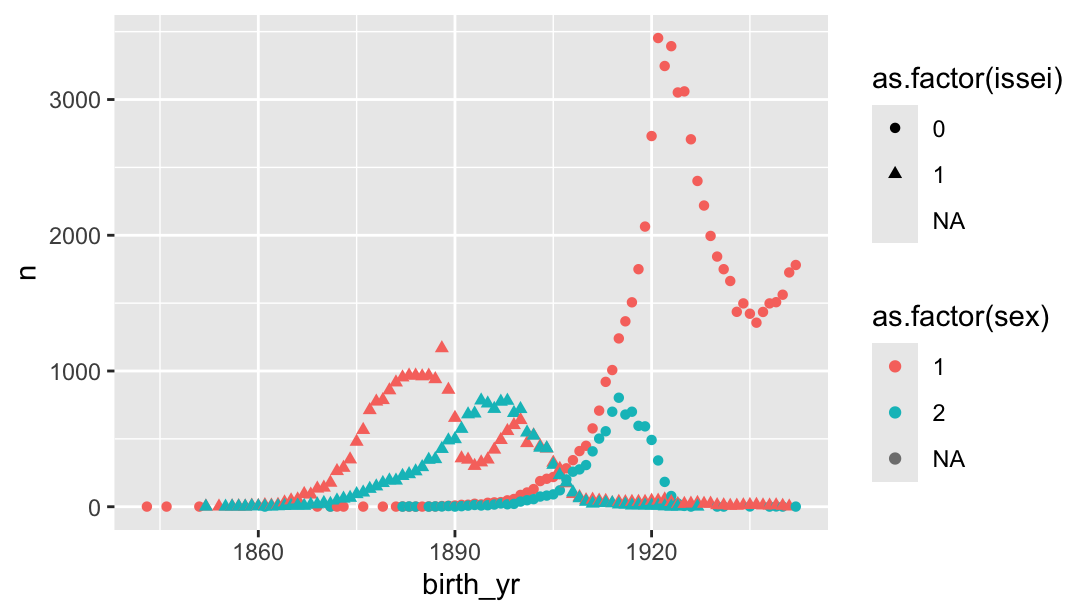
\includegraphics{figures/wra-internee-cohorts.png}

\subsection{IPUMS Census}\label{ipums-census}

\begin{itemize}
\tightlist
\item
  Decennial Census Data for years 1940, 1950, 1960, 1970, 1980, and 1990

  \begin{itemize}
  \tightlist
  \item
    Via IPUMS USA (\textbf{ruggles\_steven\_ipums\_2024?})
  \end{itemize}
\end{itemize}

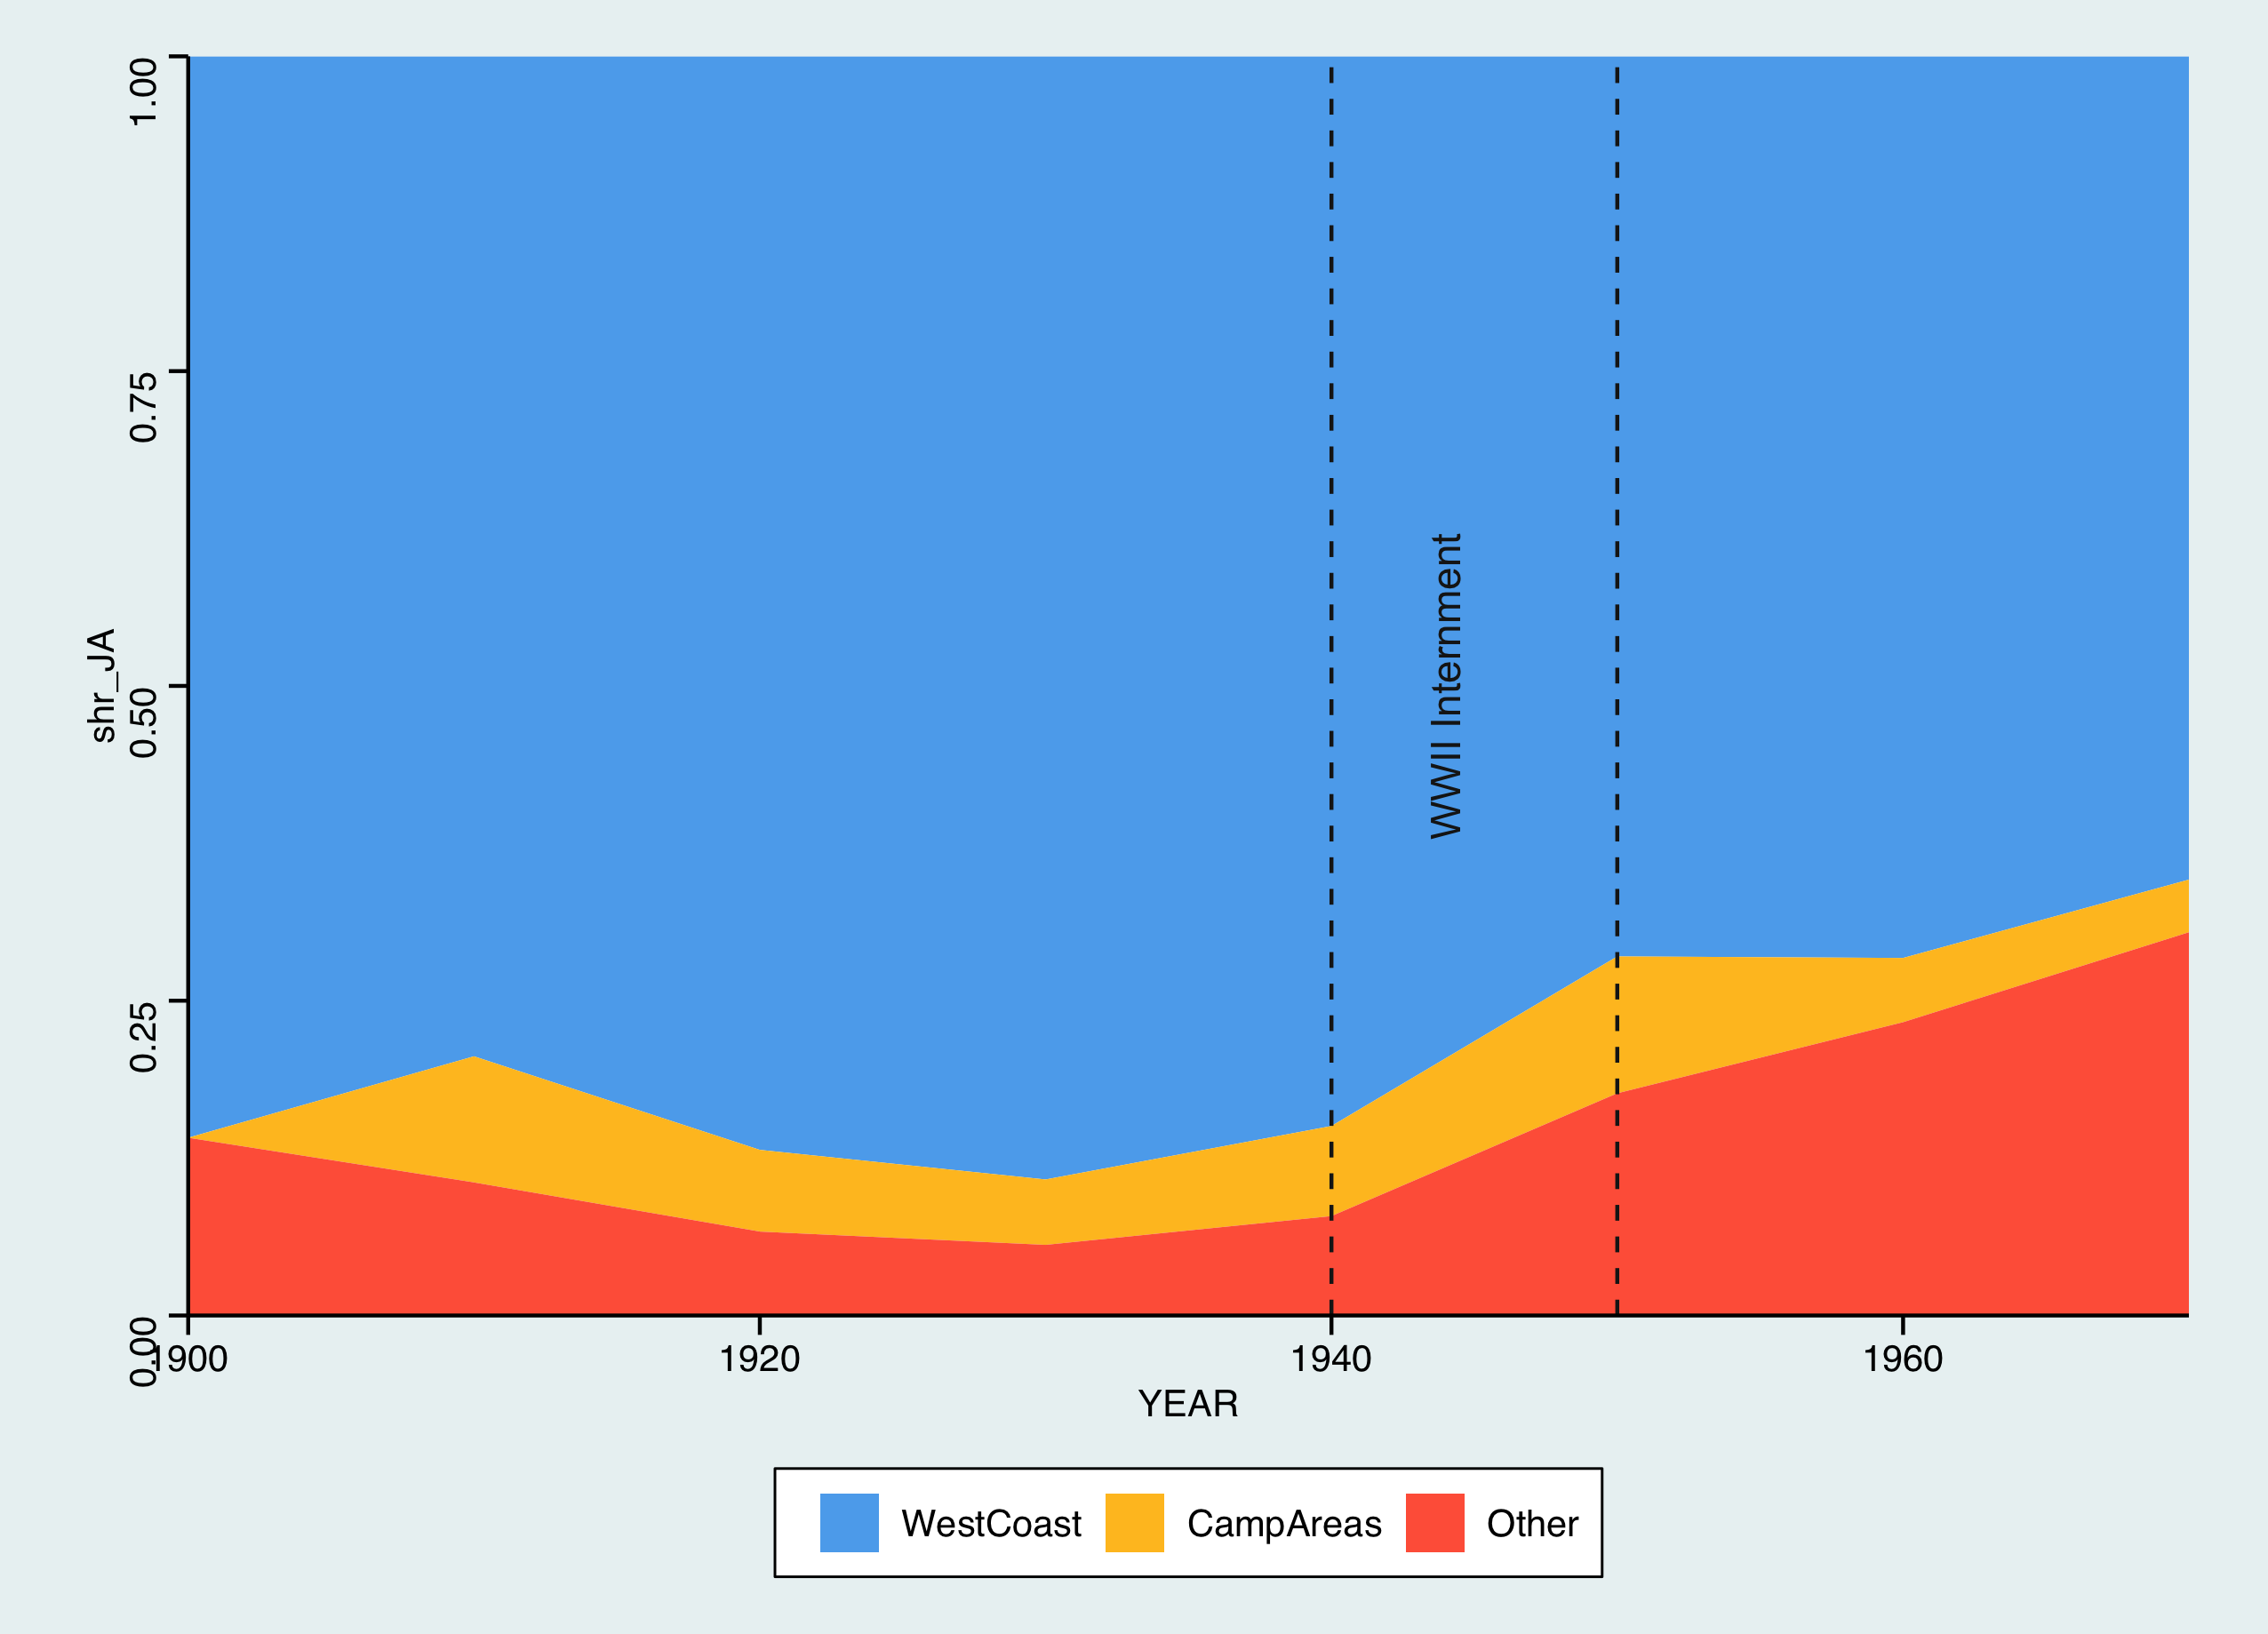
\includegraphics{figures/shareareaplot.png}

\subsection{NHGIS geo}\label{nhgis-geo}

--

\section{Methods}\label{methods}

\subsection{immigration on dist to
camps}\label{immigration-on-dist-to-camps}

\subsubsection{within cont. US migration of japanese
americans}\label{within-cont.-us-migration-of-japanese-americans}

\subsubsection{new immigration from
japan}\label{new-immigration-from-japan}

\subsection{individual-level characteristics vs
internees?}\label{individual-level-characteristics-vs-internees}

\section{Results}\label{results}

\section{Conclusion}\label{conclusion}




\end{document}
